\documentclass[aspectratio=1610,onlymath]{beamer}
% \documentclass[aspectratio=1610,onlymath,handout]{beamer}

% Macros used by all lectures, but not necessarily by excercises

%%% General setup and dependencies:

% \usetheme[ddcfooter,nosectionnum]{tud}
\usetheme[nosectionnum,pagenum,noheader]{tud}
% \usetheme[nosectionnum,pagenum]{tud}

% Increase body font size to a sane level:
\let\origframetitle\frametitle
% \renewcommand{\frametitle}[1]{\origframetitle{#1}\normalsize}
\renewcommand{\frametitle}[1]{\origframetitle{#1}\fontsize{10pt}{13.2}\selectfont}
\setbeamerfont{itemize/enumerate subbody}{size=\small} % tud defaults to scriptsize!
\setbeamerfont{itemize/enumerate subsubbody}{size=\small}
% \setbeamerfont{normal text}{size=\small}
% \setbeamerfont{itemize body}{size=\small}

\renewcommand{\emph}[1]{\textbf{#1}}

\def\arraystretch{1.3}% Make tables even less cramped vertically

\usepackage[ngerman]{babel}
\usepackage[utf8]{inputenc}
\usepackage[T1]{fontenc}

%\usepackage{graphicx}
\usepackage[export]{adjustbox} % loads graphicx
\usepackage{import}
\usepackage{stmaryrd}
\usepackage[normalem]{ulem} % sout command
% \usepackage{times}
\usepackage{txfonts}
\usepackage{array}

% \usepackage[perpage]{footmisc} % reset footnote counter on each page -- fails with beamer (footnotes gone)
\usepackage{perpage}  % reset footnote counter on each page
\MakePerPage{footnote}

\usepackage{tikz}
\usetikzlibrary{arrows,positioning,decorations.pathreplacing}
% Inspired by http://www.texample.net/tikz/examples/hand-drawn-lines/
\usetikzlibrary{decorations.pathmorphing}
\pgfdeclaredecoration{penciline}{initial}{
    \state{initial}[width=+\pgfdecoratedinputsegmentremainingdistance,
    auto corner on length=1mm,]{
        \pgfpathcurveto%
        {% From
            \pgfqpoint{\pgfdecoratedinputsegmentremainingdistance}
                      {\pgfdecorationsegmentamplitude}
        }
        {%  Control 1
        \pgfmathrand
        \pgfpointadd{\pgfqpoint{\pgfdecoratedinputsegmentremainingdistance}{0pt}}
                    {\pgfqpoint{-\pgfdecorationsegmentaspect
                     \pgfdecoratedinputsegmentremainingdistance}%
                               {\pgfmathresult\pgfdecorationsegmentamplitude}
                    }
        }
        {%TO
        \pgfpointadd{\pgfpointdecoratedinputsegmentlast}{\pgfpoint{1pt}{1pt}}
        }
    }
    \state{final}{}
}
\tikzset{handdrawn/.style={decorate,decoration=penciline}}
\tikzset{every shadow/.style={fill=none,shadow xshift=0pt,shadow yshift=0pt}}
% \tikzset{module/.append style={top color=\col,bottom color=\col}}

% Use to make Tikz attributes with Beamer overlays
% http://tex.stackexchange.com/a/6155
\tikzset{onslide/.code args={<#1>#2}{%
  \only<#1| handout:0>{\pgfkeysalso{#2}}
}}
\tikzset{onslideprint/.code args={<#1>#2}{%
  \only<#1>{\pgfkeysalso{#2}}
}}

%%% Title -- always set this first

\newcommand{\defineTitle}[3]{
	\newcommand{\lectureindex}{#1}
	\title{Theoretische Informatik und Logik}
	\subtitle{\href{\lectureurl}{#1. Vorlesung: #2}}
	\author{\href{https://iccl.inf.tu-dresden.de/web/Markus_Kr\%C3\%B6tzsch}{Markus Kr\"{o}tzsch}\\[1ex]Lehrstuhl Wissensbasierte Systeme}
	\date{#3}
	\datecity{TU Dresden}
% 	\institute{CC-By 3.0, sofern keine anderslautenden Bildrechte angegeben sind}
}

%%% Table of contents:

\RequirePackage{ifthen}

\newcommand{\highlight}[2]{%
	\ifthenelse{\equal{#1}{\lectureindex}}{\alert{#2}}{#2}%
}

\def\myspace{-0.7ex}
\newcommand{\printtoc}{
\begin{tabular}{r@{$\quad$}l}
\highlight{1}{1.} & \highlight{1}{Willkommen/Einleitung formale Sprachen}\\[\myspace]
\highlight{2}{2.} & \highlight{2}{Grammatiken und die Chomsky-Hierarchie}\\[\myspace]
\highlight{3}{3.} & \highlight{3}{Endliche Automaten}\\[\myspace]
\highlight{4}{4.} & \highlight{4}{Complexity of FO query answering}\\[\myspace]
\highlight{5}{5.} & \highlight{5}{Conjunctive queries}\\[\myspace]
\highlight{6}{6.} & \highlight{6}{Tree-like conjunctive queries}\\[\myspace]
\highlight{7}{7.} & \highlight{7}{Query optimisation}\\[\myspace]
\highlight{8}{8.} & \highlight{8}{Conjunctive Query Optimisation / First-Order~Expressiveness}\\[\myspace]
\highlight{9}{9.} & \highlight{9}{First-Order~Expressiveness / Introduction to Datalog}\\[\myspace]
\highlight{10}{10.} & \highlight{10}{Expressive Power and Complexity of Datalog}\\[\myspace]
\highlight{11}{11.} & \highlight{11}{Optimisation and Evaluation of Datalog}\\[\myspace]
\highlight{12}{12.} & \highlight{12}{Evaluation of Datalog (2)}\\[\myspace]
\highlight{13}{13.} & \highlight{13}{Graph Databases and Path Queries}\\[\myspace]
\highlight{14}{14.} & \highlight{14}{Outlook: database theory in practice}
\end{tabular}
}

\newcommand{\overviewslide}{%
\begin{frame}\frametitle{Overview}
\printtoc
\medskip

Siehe \href{\lectureurl}{course homepage [$\Rightarrow$ link]} for more information and materials
\end{frame}
}

%%% Colours:
\usepackage{xcolor,colortbl}
\definecolor{redhighlights}{HTML}{FFAA66}
\definecolor{lightblue}{HTML}{55AAFF}
\definecolor{lightred}{HTML}{FF5522}
\definecolor{lightpurple}{HTML}{DD77BB}
\definecolor{lightgreen}{HTML}{55FF55}
\definecolor{darkred}{HTML}{CC4411}
\definecolor{darkblue}{HTML}{176FC0}%{1133AA}
\definecolor{nightblue}{HTML}{2010A0}%{1133AA}
\definecolor{alert}{HTML}{176FC0}
\definecolor{darkgreen}{HTML}{36AB14}
\definecolor{strongyellow}{HTML}{FFE219}
\definecolor{devilscss}{HTML}{666666}

\newcommand{\redalert}[1]{\textcolor{darkred}{#1}}

%%% Slide layout commands:

\newcommand{\sectionSlide}[1]{
\frame{\begin{center}
\LARGE
#1
\end{center}}
}
\newcommand{\sectionSlideNoHandout}[1]{
\frame<handout:0>{\begin{center}
\LARGE
#1
\end{center}}
}

\newcommand{\mydualbox}[3]{%
 \begin{minipage}[t]{#1}
 \begin{beamerboxesrounded}[upper=block title,lower=block body,shadow=true]%
    {\centering\usebeamerfont*{block title}#2}%
    \raggedright%
    \usebeamerfont{block body}
%     \small
    #3%
  \end{beamerboxesrounded}
  \end{minipage}
}
%
\newcommand{\myheaderbox}[2]{%
 \begin{minipage}[t]{#1}
 \begin{beamerboxesrounded}[upper=block title,lower=block title,shadow=true]%
    {\centering\usebeamerfont*{block title}\rule{0pt}{2.6ex} #2}%
  \end{beamerboxesrounded}
  \end{minipage}
}

\newcommand{\mycontentbox}[2]{%
 \begin{minipage}[t]{#1}%
 \begin{beamerboxesrounded}[upper=block body,lower=block body,shadow=true]%
    {\centering\usebeamerfont*{block body}\rule{0pt}{2.6ex}#2}%
  \end{beamerboxesrounded}
  \end{minipage}
}

\newcommand{\mylcontentbox}[2]{%
 \begin{minipage}[t]{#1}%
 \begin{beamerboxesrounded}[upper=block body,lower=block body,shadow=true]%
    {\flushleft\usebeamerfont*{block body}\rule{0pt}{2.6ex}#2}%
  \end{beamerboxesrounded}
  \end{minipage}
}

% label=180:{\rotatebox{90}{{\footnotesize\textcolor{darkgreen}{Beispiel}}}}
% \hspace{-8mm}\ghost{\raisebox{-7mm}{\rotatebox{90}{{\footnotesize\textcolor{darkgreen}{Beispiel}}}}}\hspace{8mm}
\newcommand{\examplebox}[1]{%
	\begin{tikzpicture}[decoration=penciline, decorate]
		\pgfmathsetseed{1235}
		\node (n1) [decorate,draw=darkgreen, fill=darkgreen!10,thick,align=left,text width=\linewidth, inner ysep=2mm, inner xsep=2mm] at (0,0) {#1};
% 		\node (n2) [align=left,text width=\linewidth,inner sep=0mm] at (n1.92) {{\footnotesize\raisebox{3mm}{\textcolor{darkgreen}{Beispiel}}}};
% 		\node (n2) [decorate,draw=darkgreen, fill=darkgreen!10,thick, align=left,text width=\linewidth,inner sep=2mm] at (n1.90) {{\footnotesize\raisebox{0mm}{\textcolor{darkgreen}{Beispiel}}}};
	\end{tikzpicture}%
}%

\newcommand{\codebox}[1]{%
	\begin{tikzpicture}[decoration=penciline, decorate]
		\pgfmathsetseed{1236}
		\node (n1) [decorate,draw=strongyellow, fill=strongyellow!10,thick,align=left,text width=\linewidth, inner ysep=2mm, inner xsep=2mm] at (0,0) {#1};
	\end{tikzpicture}%
}%

\newcommand{\defbox}[1]{%
	\begin{tikzpicture}[decoration=penciline, decorate]
		\pgfmathsetseed{1237}
		\node (n1) [decorate,draw=darkred, fill=darkred!10,thick,align=left,text width=\linewidth, inner ysep=2mm, inner xsep=2mm] at (0,0) {#1};
	\end{tikzpicture}%
}%

\newcommand{\theobox}[1]{%
	\begin{tikzpicture}[decoration=penciline, decorate]
		\pgfmathsetseed{1240}
		\node (n1) [decorate,draw=darkblue, fill=darkblue!10,thick,align=left,text width=\linewidth, inner ysep=2mm, inner xsep=2mm] at (0,0) {#1};
	\end{tikzpicture}%
}%

\newcommand{\anybox}[2]{%
	\begin{tikzpicture}[decoration=penciline, decorate]
		\pgfmathsetseed{1240}
		\node (n1) [decorate,draw=#1, fill=#1!10,thick,align=left,text width=\linewidth, inner ysep=2mm, inner xsep=2mm] at (0,0) {#2};
	\end{tikzpicture}%
}%


\newsavebox{\mybox}%
\newcommand{\doodlebox}[2]{%
\sbox{\mybox}{#2}%
	\begin{tikzpicture}[decoration=penciline, decorate]
		\pgfmathsetseed{1238}
		\node (n1) [decorate,draw=#1, fill=#1!10,thick,align=left,inner sep=1mm] at (0,0) {\usebox{\mybox}};
	\end{tikzpicture}%
}%


\defineTitle{24}{Gödel, Turing und der ganze Rest}{13. Juli 2018}

\begin{document}

\maketitle

\frame{\label{frame_goedel}\begin{center}
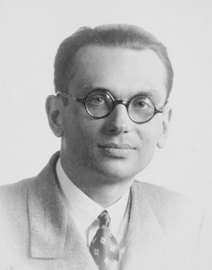
\includegraphics[height=5cm]{images/Goedel.jpg}

\LARGE
Kurt Gödel
\end{center}}

% Goedels Unvollstaendigkeitssaetze (mit vagen Formulierungen), ev. erstmal nur UV1
\begin{frame}\frametitle{Der 1. Gödelsche Unvollständigkeitssatz}

\theobox{Satz (Gödel, 1931): Jedes konsistente formale System, in dem eine gewisse Menge elementarer Arithmetik
dargestellt werden kann, ist unvollständig in Bezug auf die Beweisbarkeit von Sätzen der
elementaren Arithmetik.
}\bigskip

\emph{Relevante Begriffe:}
\begin{itemize}
\item \alert{Formales System:} Ein implementierbares Verfahren, mit dem man Theoreme endlich beweisen kann
\item \alert{Konsistent:} Man kann niemals eine Aussage und ihr Gegenteil beweisen.
\item \alert{Gewisse Menge Arithmetik:} Kodierung konkreter natürlicher Zahlen und deren korrekte Addition, Subtraktion, Multiplikation und Vergleich
\item \alert{Unvollständig:} Es gibt Sätze, die weder bewiesen noch widerlegt werden können
\end{itemize}

\end{frame}

\begin{frame}\frametitle{Beispiele}

\examplebox{Beispiel: Natürliche Zahlen und einfache Rechenregeln können mit einer prädikatenlogischen Theorie definiert werden. Mit Resolution kann man daraus korrekte neue Schlüsse ziehen. Laut Gödels erstem Satz kann man auf diese Art aber niemals alle wahren Aussagen der Arithmetik beweisen, außer wenn die Theorie widersprüchlich ist.}

\redalert{Keine prädikatenlogische Theorie kann die elementare Arithmetik vollständig beschreiben.}\pause\bigskip

\examplebox{Beispiel: Die moderne Mathematik basiert auf der Mengenlehre von Zermelo-Fraenkel unter Hinzunahme des Auswahlaxioms. Dieses formale System heißt \alert{ZFC}. Es ist klar definiert, was ein korrekter mathematischer Beweis in ZFC ist. Laut Gödels erstem Satz gibt es also wahre Aussagen über elementare Arithmetik, die nicht in ZFC bewiesen werden können.}

\end{frame}

\begin{frame}\frametitle{Gödels 2. Unvollständigkeitssatz}

Gödel kam direkt zu einer weiteren Schlussfolgerung:\medskip

\theobox{Satz: Jedes konsistente formale System, in dem eine gewisse Menge elementarer Arithmetik
dargestellt werden kann, kann nicht seine eigene Konsistenz beweisen.
}\bigskip

\emph{Auch hier gibt es einige vage Punkte:}
\begin{itemize}
\item Was ist \alert{"`eine gewisse Menge elementarer Arithmetik"'}?
\item Was genau bedeutet \alert{"`seine eigene Konsistenz beweisen"'}?
\end{itemize}

\end{frame}

\begin{frame}\frametitle{Konsistenz beweisen}

\emph{Konsistenz bedeutet formal:}\medskip

"`Für alle Sätze $F$ gilt: es gibt keinen Beweis für $F$ oder es gibt keinen Beweis für $\neg F$."'
\bigskip

\begin{itemize}
\item Um das ausdrücken zu können, muss das System über die im eigenen System möglichen Beweise reflektieren können
\item Diese Idee ist verwandt mit der Intuition, dass man in Arithmetik universelle Turingmaschinen kodieren kann: die Beweise eines Systems sind letztlich die akzeptierenden Läufe einer TM
\item Man benötigt dazu etwas mehr Arithmetik als für den Beweis des 1. Unvollständigkeitssatzes (Details sparen wir uns)
\end{itemize}

\end{frame}

\begin{frame}\frametitle{Beweis des 2. Unvollständigkeitssatzes}

\alert{Gödels Argument für seinen 1. Unvollständigkeitssatz (vereinfacht):}
\anybox{strongyellow}{
Gödel definiert eine mathematische Formel $F$, welche ausdrückt:\\[1ex]
\narrowcentering{\alert{"`$F$ ist wahr genau dann wenn $F$ nicht beweisbar ist."'}}\smallskip

\begin{itemize}
\item Wenn $F$ beweisbar wäre, dann ist sie wahr und also nicht beweisbar -- Widerspruch
\item Also ist $F$ nicht beweisbar, und damit wahr\qed
\end{itemize}}

Es stellt sich heraus: mit einer "`gewissen Menge Arithmetik"' kann man diese Argumentation komplett im System darstellen!\medskip\pause

\redalert{Warum ist diese Argumentation dann nicht schon ein Beweis für $F$?}\pause\bigskip

\alert{Weil wir die Annahme verwenden, dass das System konsistent ist.}
\begin{itemize}
\item Wenn wir dies beweisen könnten, so wäre auch $F$ beweisbar.
\item Aber laut 1. Unvollständigkeitssatz ist $F$ nicht beweisbar.
\end{itemize}
Also kann die Konsistenz des Systems nicht beweisbar sein. \qed

\end{frame}

\begin{frame}\frametitle{Beispiele}

\examplebox{Beispiel: Es gibt keinen elementaren arithmetischen Beweis für die Widerspruchsfreiheit der Peano-Arithmetik. Man kann deren Konsistenz aber leicht im 
stärkeren System ZFC beweisen.}\bigskip\pause

\examplebox{Beispiel: Es ist nicht möglich, die Widerspruchsfreiheit der modernen Mathematik
(ZFC) aus sich selbst heraus zu beweisen. Auch das kann man allerdings in mächtigeren Systemen erreichen.}\bigskip\pause

\emph{Anmerkung:} Dadurch wird die Mathematik nicht in eine Sinnkrise gestürzt. Selbst wenn
man die Konsistenz von ZFC in ZFC beweisen könnte wäre dies sicherlich kein starkes Argument für ZFC. Mathematische Systeme erhalten ihre Bedeutung niemals aus sich selbst heraus.

\end{frame}

\begin{frame}\frametitle{Der universelle elektronische Mathematiker}

Oder: "`Hilberts Programm als Turingmaschine"'
% Noch eine Konsequenz von Gödels 2. Satz:
% \redalert{Konkrete Fragen der Informatik sind für die moderne Mathematik unlösbar!}
\bigskip

\emph{Skizze einer Turingmaschine:}
\begin{itemize}
\item Bilde systematisch der Reihe nach alle möglichen Beweise der modernen Mathematik (System ZFC)
\item Halte sobald ein Beweis für die Aussage "`0=1"' auftaucht
\end{itemize}
\alert{Hält diese Turingmaschine?}\pause
\begin{itemize}
\item Ja, wenn ZFC inkonsistent ist
\item Nein, wenn ZFC konsistent ist
\end{itemize}\pause
\bigskip

\redalert{$\leadsto$ Vermutlich hält die TM nicht, aber die moderne Mathematik kann das nicht beweisen.}\pause\medskip

\emph{Anmerkung:} Es gibt eine bekannte TM mit 7910 Zuständen, die sich so verhält [Yedidia \& Aaronson 2016] und sogar eine mit nur 1919 Zuständen [O’Rear, 2016]

\end{frame}

\begin{frame}\frametitle{Konsequenzen}

Wir haben Turing-Mächtigkeit und Unentscheidbarkeit in vielen Formalismen gezeigt -- jedes davon erlaubt die Konstruktion universeller Mathematiker!
\bigskip

\emph{Es gibt konkrete Beispiele für}
\begin{itemize}
\item WHILE-Programme,
\item Python-Programme,
\item Typ-0-Grammatiken,
\item PCP-Instanzen,
\item diophantische Gleichungen,
\item prädikatenlogische Theorien,
\item \ldots
\end{itemize}
deren Halten/Leerheit/Lösbarkeit/Erfüllbarkeit nicht durch die übliche Mathematik (=ZFC) bewiesen oder widerlegt werden kann\\[-0.5ex]
{\tiny zumindest falls die übliche Mathematik konsistent ist}

\end{frame}

\begin{frame}\frametitle{Hilberts 10. Problem, revisited}

\alert{Hilbert:} "`\ldots man soll ein Verfahren angeben, nach welchem sich mittels einer endlichen Anzahl von Operationen entscheiden lässt, ob die Gleichung in ganzen rationalen Zahlen lösbar ist."'
\bigskip\pause

\alert{Turing:} Es gibt Probleme, die durch kein automatisches Verfahren lösbar sind.
\medskip\pause

\alert{Gödel:} Es gibt konstruierbare Beispiele konkreter arithmetischer Sätze, deren Gültigkeit nicht in der modernen Mathematik bewiesen oder widerlegt werden kann.
\medskip\pause

\alert{Matiyasevich/Robinson/Davis/Putnam:} Die Lösbarkeit diophantischer Gleichungen ist
unentscheidbar.
\medskip\pause

\alert{Alle zusammen:} Es gibt also sogar konkrete diophantische Gleichungen, deren Lösbarkeit nicht in der modernen Mathematik bewiesen oder widerlegt werden kann.\medskip\pause

{\tiny
\emph{Aber:} Die Lösbarkeit jeder konkreten diophantischen Gleichung wird durch irgendein Programm entschieden (wir wissen nur oft nicht, welches, bzw. können seine Korrektheit nicht in ZFC mathematisch beweisen).

}

\end{frame}

\sectionSlide{Besprechung Lehrevaluation}


\sectionSlide{Ausblick}

% Second-Order Logic (siehe Advanced Logics)
\begin{frame}\frametitle{Logik höherer Ordnung}

Prädikatenlogik ist genau genommen \alert{Prädikatenlogik erster Stufe}.
\bigskip

\emph{Hintergrund:}
\begin{itemize}
\item Erste Stufe: Quantoren beziehen sich auf Domänenelemente\smallskip

\examplebox{Beispiel: "`Jede natürliche Zahl $n$ hat einen Nachfolger $s(n)$"'}
% \[ \forall x.(\textsf{natnum}(x)\to\textsf{natnum}(s(x))) \]
\item Zweite Stufe: Quantoren beziehen sich auf Prädikate\smallskip

\examplebox{Beispiel: "`Für jede Menge $M$ gilt: Enthält $M$ die Zahl $0$ und mit jeder natürlichen Zahl $n$ auch stets deren Nachfolger $s(n)$, so enthält $M$ alle natürlichen Zahlen."'}
\end{itemize}\bigskip

\emph{Logik zweiter Ordnung:}
\begin{itemize}
\item Ausdrucksstärker; kann z.B. die natürlichen Zahlen exakt charakterisieren
\item Schwieriger: kein vollständiges und korrektes \ghost{Beweisverfahren}
\end{itemize}

$\leadsto$ siehe Vorlesung \redalert{Advanced Logic}

\end{frame}

% Complexity Theory
\begin{frame}\frametitle{Komplexitätstheorie}

Wesentliche Grundlagen der klassischen Komplexitätslehre wurden hier schon behandelt
\bigskip

\emph{Weiterführende Themen (Beispiele):}
\begin{itemize}
\item Hierarchietheoreme: Kann man mit mehr Zeit/Speicher wirklich mehr berechnen?
\item Relative Komplexität: Orakel
\item Komplexitäten unterhalb von P: Schaltkreise als Rechenmodell
\item Rechnen mit Zufall: Randomisierte Komplexität
\item Einführung in Quantencomputer
\item \ldots
\end{itemize}

$\leadsto$ siehe Vorlesung \redalert{Complexity Theory} (Wintersemester)

\end{frame}

% Database Theory
\begin{frame}\frametitle{Datenbanktheorie}

Die Theorie der Datenbanken ist ein wichtiges Anwendungsgebiet für
viele Themen aus theoretischer Informatik und Logik\bigskip

\emph{Weiterführende Themen (Beispiele):}
\begin{itemize}
\item Anfragesprachen vergleichen bzgl. Komplexität und Ausdrucksstärke
\item Relationales Kalkül (=Prädikatenlogik)
\item Datalog: rekursive Anfragesprache, Fragment der Logik zweiter Stufe
\item Graph-Anfragen: Erreichbarkeit und Co. berechnen
\item Anfragen unter Berücksichtigung von Constraints
\item \ldots
\end{itemize}

$\leadsto$ siehe Vorlesung \redalert{Database Theory} (Sommersemester)

\end{frame}

% Verifikation
\begin{frame}\frametitle{Verifikation}

Programm- und Hardwareverifikation ist eine wichtige Anwendung logischer Methoden
\bigskip

\emph{Weiterführende Themen (Beispiele):}
\begin{itemize}
\item Modellierung reaktiver Systeme: Transaktionssysteme
\item Automatenmodelle zur Darstellung verifizierbarer Eigenschaften
\item Lineare Temporallogik (LTL) und Computation Tree Logic (CTL)
\item Probabilistische und zeitgesteuerte Automaten
\item \ldots
\end{itemize}

$\leadsto$ siehe Vorlesung \redalert{Model Checking}

\end{frame}

% Quantum Computation -- advertise Aaronson's talk
% \begin{frame}\frametitle{Quantencomputer}
% 
% Aktives Gebiet der theoretischen Informatik, speziell der Komplexitätstheorie\bigskip\pause
% 
% % Zurzeit keine Vorlesung an TUD, aber:\medskip
% 
% % \emph{Eingeladener Vortrag:}\\
% {\large Quantum Computing and the Limits of the Efficiently Computable}\\
% \alert{Scott Aaronson}, The University of Texas at Austin\\
% Montag, 28. August 2017, 14:00 -- APB E023
% \bigskip
% 
% {\footnotesize
% I'll offer a crash course on quantum computing, which seeks to exploit the strange rules of
% quantum physics to solve certain problems dramatically faster than we know how to solve
% them with any existing computer. I promise no hype: just a sober summary of how a quantum
% computer would actually work (hint: it's not just by "trying every possible answer in parallel"), for
% which problems quantum computers are and aren't expected to provide an advantage, and the
% current status of the effort to make quantum computing practical. I'll also say something about
% the ultimate physical limits of computation, and about speculative proposals for going beyond
% even quantum computers.
% 
% }
% \smallskip
% 
% \tiny
% \url{https://cfaed.tu-dresden.de/cfaed-seminar-series/scott-aaronsons-talk}
% 
% \end{frame}

% Knowledge representation: tractability and decidability, siehe z.B. Beschreibungslogik
\begin{frame}\frametitle{Symbolische Wissensrepräsentation}

Anwendungsgebiet der formalen Logik, bei dem menschliches Wissen logisch kodiert und automatisch ausgewertet wird
\bigskip

\emph{Weiterführende Themen (Beispiele):}
\begin{itemize}
\item Entwicklung logischer Sprachen, für die Schlussfolgerung (effizient) entscheidbar ist
\item Meist durch Einschränkung auf Teilmengen der Prädikatenlogik, z.B. bei Beschreibungslogiken
\item Ontologien: logische Wissensmodelle
\item Entwicklung effizienter Ableitungsalgorithmen und Implementierungen
\item \ldots
\end{itemize}

$\leadsto$ verschiedene Vorlesungen, z.B. \redalert{Description Logics}

\end{frame}

% The Semantic Web
\begin{frame}\frametitle{Semantic Web \& Datenaustausch}

Anwendungsgebiet zwischen Datenbanken, Wissensrepräsentation und Webtechnologie
\bigskip

\emph{Weiterführende Themen (Beispiele):}
\begin{itemize}
\item Standards zur Kodierung von Fakten und Schemainformationen: RDF, OWL, \ldots
\item Informationsintegration in (Web)Graphdatenbanken
\item Anfragesprachen: SPARQL und ontologiebasierte Anfragen
\item Anwendungen (z.B. Wikidata)
\item \ldots
\end{itemize}

$\leadsto$ siehe Vorlesungen \redalert{Knowledge Graphs} (Wintersemester), \redalert{Semantic Web Technologies}

\end{frame}

\sectionSlide{Forschung (und studentische Arbeiten)}

\begin{frame}\frametitle{Kernthemen der Professur WBS}\pause

\emph{Wissensrepräsentation:} \alert{Wie kann menschliches Wissen digital dargestellt werden?}
\begin{itemize}
\item Herausforderung: Flexibilität vs. Nutzbarkeit
\item Herausforderung: Ausdrucksstärke vs. Verarbeitungskomplexität
\item Schwerpunkt: logische Ontologie- und Anfragesprachen (Regeln, DLs, \ghost{Graph-Queries, \ldots)}
\end{itemize}\medskip\pause

\emph{Wissensverarbeitung:} \alert{Wie kann dieses Wissen automatisch genutzt werden?}
\begin{itemize}
\item Herausforderung: theoretische Komplexität $\neq$ praktische Performance
\item Herausforderung: prinzipielles Verfahren $\neq$ implementierbarer Algorithmus
\item Schwerpunkt: Logisches Schließen, Anfragebeantwortung über großen Daten
\end{itemize}\medskip\pause

\emph{Wissensmanagement:} \alert{Wie können diese Ergebnisse praktisch genutzt werden?}
\begin{itemize}
\item Herausforderung: konkrete Märkte und Nutzer?
\item Herausforderung: benötigt mehr als eine Kerntechnologie
\item Schwerpunkt: Wikidata, Wissensgraphen, Ontologien in Life Sciences
\end{itemize}

\end{frame}

\begin{frame}\frametitle{Beispiele für BSc/MSc-Themen}

\emph{Wissensrepräsentation:} \alert{Wie kann menschliches Wissen digital dargestellt werden?}
\begin{itemize}
\item Weiterentwicklung aktueller Schließverfahren
\item Verallgemeinerung neuer Ideen unter Anleitung
\item \ldots
\end{itemize}\medskip

\emph{Wissensverarbeitung:} \alert{Wie kann dieses Wissen automatisch genutzt werden?}
\begin{itemize}
\item Ontologieschließen: Aufgaben Übersetzen und mit Regel-Engine lösen
\item Regelanalyse: Implementierung kürzlich erfundener Verfahren
\item Evaluation: Vergleich vorgeschlagener Algorithmen
\end{itemize}\medskip

\emph{Wissensmanagement:} \alert{Wie können diese Ergebnisse praktisch genutzt werden?}
\begin{itemize}
\item Analyse der Wikidata-Nutzung: Logs von SPARQL-Anfragen analysieren
\item IDEs zur Ontologieentwicklung: Design, Prototypen
\item Neue Anwendungen, z.B. Informationsextraktion mit logischen Regeln
\end{itemize}

\end{frame}


\sectionSlide{Zusammenfassung}

\begin{frame}\frametitle{Übersicht}


\emph{Berechenbarkeit:} Turingmaschinen, LOOP/WHILE, Entscheidbarkeit, Beispielprobleme (Halten, PCP)
\bigskip

\emph{Komplexität:} NP, PSpace, Many-One-Reduktionen, Übersicht weiterer wichtiger Klassen
\bigskip

\emph{Logik:} Aussagenlogik (SAT), QBF, Prädikatenlogik, Resolution (mit vielen Teilschritten), Herbrandmodelle, Datalog
\bigskip

\emph{Bonusmaterial:} Gödel, Metamathematik, SQL, Geschichte und Geschichten

\end{frame}

\begin{frame}\frametitle{Querschnittsthemen}

\begin{center}
\large

Informatik ist überall dort, wo gerechnet wird\pause\\[4ex]

Rechnen = Schlussfolgern\pause\\[4ex]

Beweisen -- Nachvollziehen -- Verstehen\pause\\[4ex]

\end{center}

\end{frame}


\begin{frame}\frametitle{The End}

\bigskip
\begin{center}
{\Huge Fragen?}
\end{center}
\bigskip\bigskip

\anybox{yellow}{
Was erwartet uns als nächstes?
\begin{itemize}
\item Zweites Repetitorium
\item Angestrengte Klausurvorbereitung (inklusive Besprechung Probeklausur)
\item Betreute Lernräume
\item Klausur
\end{itemize}
}

\end{frame}


\begin{frame}[t]\frametitle{Literatur und Bildrechte}

\alert{Literatur}\bigskip

\begin{itemize}
\item A. Yedidia, S. Aaronson: \emph{A Relatively Small Turing Machine Whose Behavior Is Independent of Set Theory.} Complex Systems 25(4), 2016.
\item S. O'Rear: \emph{Metamath Turing Machines.} \url{https://github.com/sorear/metamath-turing-machines}
\end{itemize}

\alert{Bildrechte}\bigskip

Folie \ref{frame_goedel}: Fotografie um 1926, gemeinfrei

\end{frame}


\end{document}
